\documentclass[11pt]{article}

\usepackage[margin=1.0in]{geometry}
\usepackage{fullpage}
\usepackage{url}
\usepackage{paralist}
\usepackage[pdftex]{graphicx}
\usepackage{epstopdf}
\usepackage[small]{caption}
\usepackage{subfig}
\usepackage{multirow}

\usepackage{color}


% The xxx tag is intended to denote urgent text that needs addressing.
% The meh tag is intended to highlight text that needs some loving or which
% we're not sure should make primetime
\newcommand{\xxx}[1]{{\bf \color{red} #1}}
\newcommand{\meh}[1]{{\bf \color{blue} #1}}
\newcommand\T{\rule{0pt}{3ex}}
\newcommand\B{\rule[-1.2ex]{0pt}{0pt}}

\title{Building a Visual Vocabulary Through Object Classification}
\author{Rob Goeddel \and Lauren Hinkle \and James Kirk \and Aaron Mininger}
\date{}

\begin{document}
\maketitle



\begin{abstract}
Interaction between robots and humans is a rapidly growing area of research.
Of particular interest is the desire to interact with robots or agents using
natural language. This gives humans a more natural and effective way of teaching,
commanding, and interacting with robotic agents or computers. Our work is
designed to process images and provide descriptions of objects that can then be
used in interactions with humans. We use images from an RGB-D camera in order to
classify properties of objects including size, shape, and color. These
descriptions are then fed into a higher-level agent which handles the human
interaction. We specifically use a simple I-Spy game to allow users to refer to
objects using descriptions in natural language.
\end{abstract}


\section{Introduction}
%\xxx{Problem description and motivation. Why do you want to solve this
%    problem? What's the impact if you can solve this problem?}
Language is a powerful tool that is just coming into its own as the human
interface for various systems. Apple's Siri is an excellent example of this,
making interaction with your phone intuitive, easy, and efficient. Robotic
systems in AI can also benefit from greater understanding of language. Such
knowledge could allow a human to command or teach a robot agent in a more natural
way. Take, for example, a robotic arm system with knowledge of only several nouns
and actions: cup, sink, grab/move object, and turning on/off the sink, and the
spatial concept of in. Through language, the robot could then be taught the new
action of ``filling a cup'', which means to put the cup in the sink and turn on
the sink. Even though the robot has never seen anyone fill a cup before, now it
should be able to do so itself. Furthermore, the agent could generalize the
concept to new items, like a bowl. This is a powerful way for an agent to learn
from a human, without requiring expert instructors.

Our goal is to leverage machine learning techniques in order to train a system
to know a small vocabulary of nouns, adjectives, and actions. As a proof of
concept, we want to be able to play the children's game ``I spy'' with a robotic
arm. The arm's ``eyes'' will be a Microsoft Kinect (or, with some small
probability, a stereo camera rig) capable of returning RGB-D data for
classification. A collection of objects will be placed in the view of the camera,
and a person will give a description of one of the objects. The agent will then
select the object that matches that description using the robot arm.

This work is planned to be incorporated into a larger project which includes
teaching the agent new concepts and actions as described above. Such a project
relies on having symbolic information provided by our work through object
segmentation and classification. The low level features provided by our system
can be analyzed and combined in order to build new concepts like object
categories (like blocks and balls) or object properties (all bananas are yellow).
Such reasoning and concept generalization is essential for agents that interact
in novel situations. These capabilities could be used on service tasks or with
non-robotic systems where a verbal interface offers improvements in efficiency,
safety, etc.


\section{Related Work}
%\xxx{What are existing methods? What are the state-of-the-art methods for this
%    problem? How is your approach different from the related work?}

Object classification is a problem that appears throughout a variety of
applications, ranging from law enforcement to manufacturing. While historic
efforts have focused on the recognition problem, that is, finding a known object
in a scene, more recent work has emphasized the more general problem of
classifying objects into generic groups by type~\cite{huber2004parts}. For example,
we might be interested in identifying vehicles as bikes, motorcycles, trucks,
cars, etc. Work by~\cite{nilsback2006visual} and~\cite{gehler2009feature}, among
others, has shown that powerful classifiers may be constructed through boosting
or similar across simple feature-specific classifiers such as color, shape, etc.

Recent popularization of sensors that combine both image and depth information
like the Microsoft Kinect inexpensively provide richer sensory information. The
addition of depth can help disambiguate situations that would be very difficult
with a normal camera image alone. Depth can make the determination of an object’s
underlying geometry much easier, leading to better identification
~\cite{marton2010hierarchical}.
Previous work has successfully incorporated such cameras (often called RGBD
cameras) with object recognition in indoors domains featuring common household
objects~\cite{marton2010hierarchical, lai2011sparse}.

A different approach to this problem is learning words that describe different
areas of the feature space, which can then be combined to describe classes of
objects. Research in this area focuses on learning simple, physically observable,
words with the intent of using these simple descriptors to learn more complex
nouns and relationships. Of particular popularity is an approach focused on
learning colors and shapes of small objects using sensory data
~\cite{zambuto2010visually, roy2002learning}. Additional approaches focus on
learning entities in the environment through interaction with
them~\cite{gold2009robotic}. These approaches all focus on interaction with
physical objects to discover qualities about them.

Although the types of words learned in these works is similar, the approaches and
end-goals vary. Semantic clustering~\cite{zambuto2010visually}, decision trees
~\cite{gold2009robotic}, bag of word models~\cite{roy2002learning} are all used
in the learning algorithms. This prior work focuses mostly on visual
classification and the corresponding vocabulary.

Though our work will not extend dramatically on this concept, our long term
trajectory will focus more on the complex action space, previously less explored.
This project lays the groundwork for developing an action-space, both for
learning said actions as well as learning objects upon which to act.

\section{Methodology}
%\xxx{How are you going to solve this problem? Why should the proposed method
%    work? Provide technical details of your approach if you are proposing a
%    novel method.}

Our approach will use supervised learning techniques to generate a description
of each object. First, we will gather our training data by collecting a number
of RGB-D images from the camera featuring various types and positions of objects.
Each image will be run through a segmentation process to isolate every object in
the scene. Each object will be manually given a label describing its color,
shape, and size. From these segmentations we will extract a useful feature vector
for each attribute. One of the main challenges for good object classification
will be designing a diverse and robust feature space to recognize the object
characteristics we are interested in. Color presents easy features such as RGB
and HSV descriptions. Volume computations and bounding box dimensions based on
relations to the other objects in the scene can give us scale information
necessary for estimating relative size. Shape is a more complex matter,
especially given the noise seen in the Kinect data. We plan on exploring
spherical harmonics, edge/corner features, and features based on projected
models of missing data (for example, symmetry) to correctly identify shapes.
Once the features are extracted, we need to use a machine learning algorithm to
perform the classification. We decided to use the liblinear SVM ~\cite{LIBLINEAR}
because it is widely used, powerful, reliable, and performs well for
classification tasks. We are specifically using multiclass approach because we
have attributes like color which can take on several discrete values.

For object identification we will do a similar process to segment each object in
the camera's image. That object's position in 3D space will be determined using
both the pixel coordinate and the depth value. The features will then be
extracted and run through our SVM's using the models created with the training
data. This will give us a bag of words description for each object in the scene.
This description, along with the position, will be given as input to a Soar
agent. Soar is a cognitive architecture that will be responsible for the
high-level reasoning and language processing. Our Soar agent will interpret the
commands given by the users, determine which object is being described, and give
the appropriate commands to the robotic arm.


\section{Experimental Results}

\subsection{Data Collection and Training}
We have acquired a large variety of children's foam blocks in many shapes, sizes,
and colors to act as our objects for classification. A small subset of the
blocks can be seen in Figure~\ref{fig:blocks}. Additionally we have collected 
more familiar objects to test our classifier on, demonstrating the ability of 
the system to abstract general shapes to real world objects. Some of these 
objects can be seen in Figure \meh{figure}. The foam of the blocks is an
ideal material to work with as it
\begin{inparaenum}[(1)]
\item has a smooth, matte finish,
\item comes in a variety of distinct colors, and
\item is deformable enough to be grabbed by the arm but still retain its
shape.
\end{inparaenum}


Our system, seen in figure \meh{screenshot}, segments objects found in the 
predefined play area and labels them with the most confident shape, size, and 
color.  Additionally a user can train new shapes, colors, and sizes by simply 
clicking on that image and supplying the relevant label.  This is sufficient 
for creating a large number of training samples, preferably at different 
positions and orientations.  This method is not efficient for generating a 
large number of training samples of many different objects, so we collected a 
training dataset of footage of the foam blocks at numerous positions and angles throughout the play area which were then segmented and labeled with relevant 
descriptors.

\begin{figure}
\centering
\caption{Our distribution of real-world color data in hue and saturation
    dimensions. Point colors correspond with the ground truth color labeling,
    so true red examples are shown as red +s.}
\label{fig:colordata}
\end{figure}

\begin{figure}[h!]
\centering
\subfloat[Foam Blocks] {
    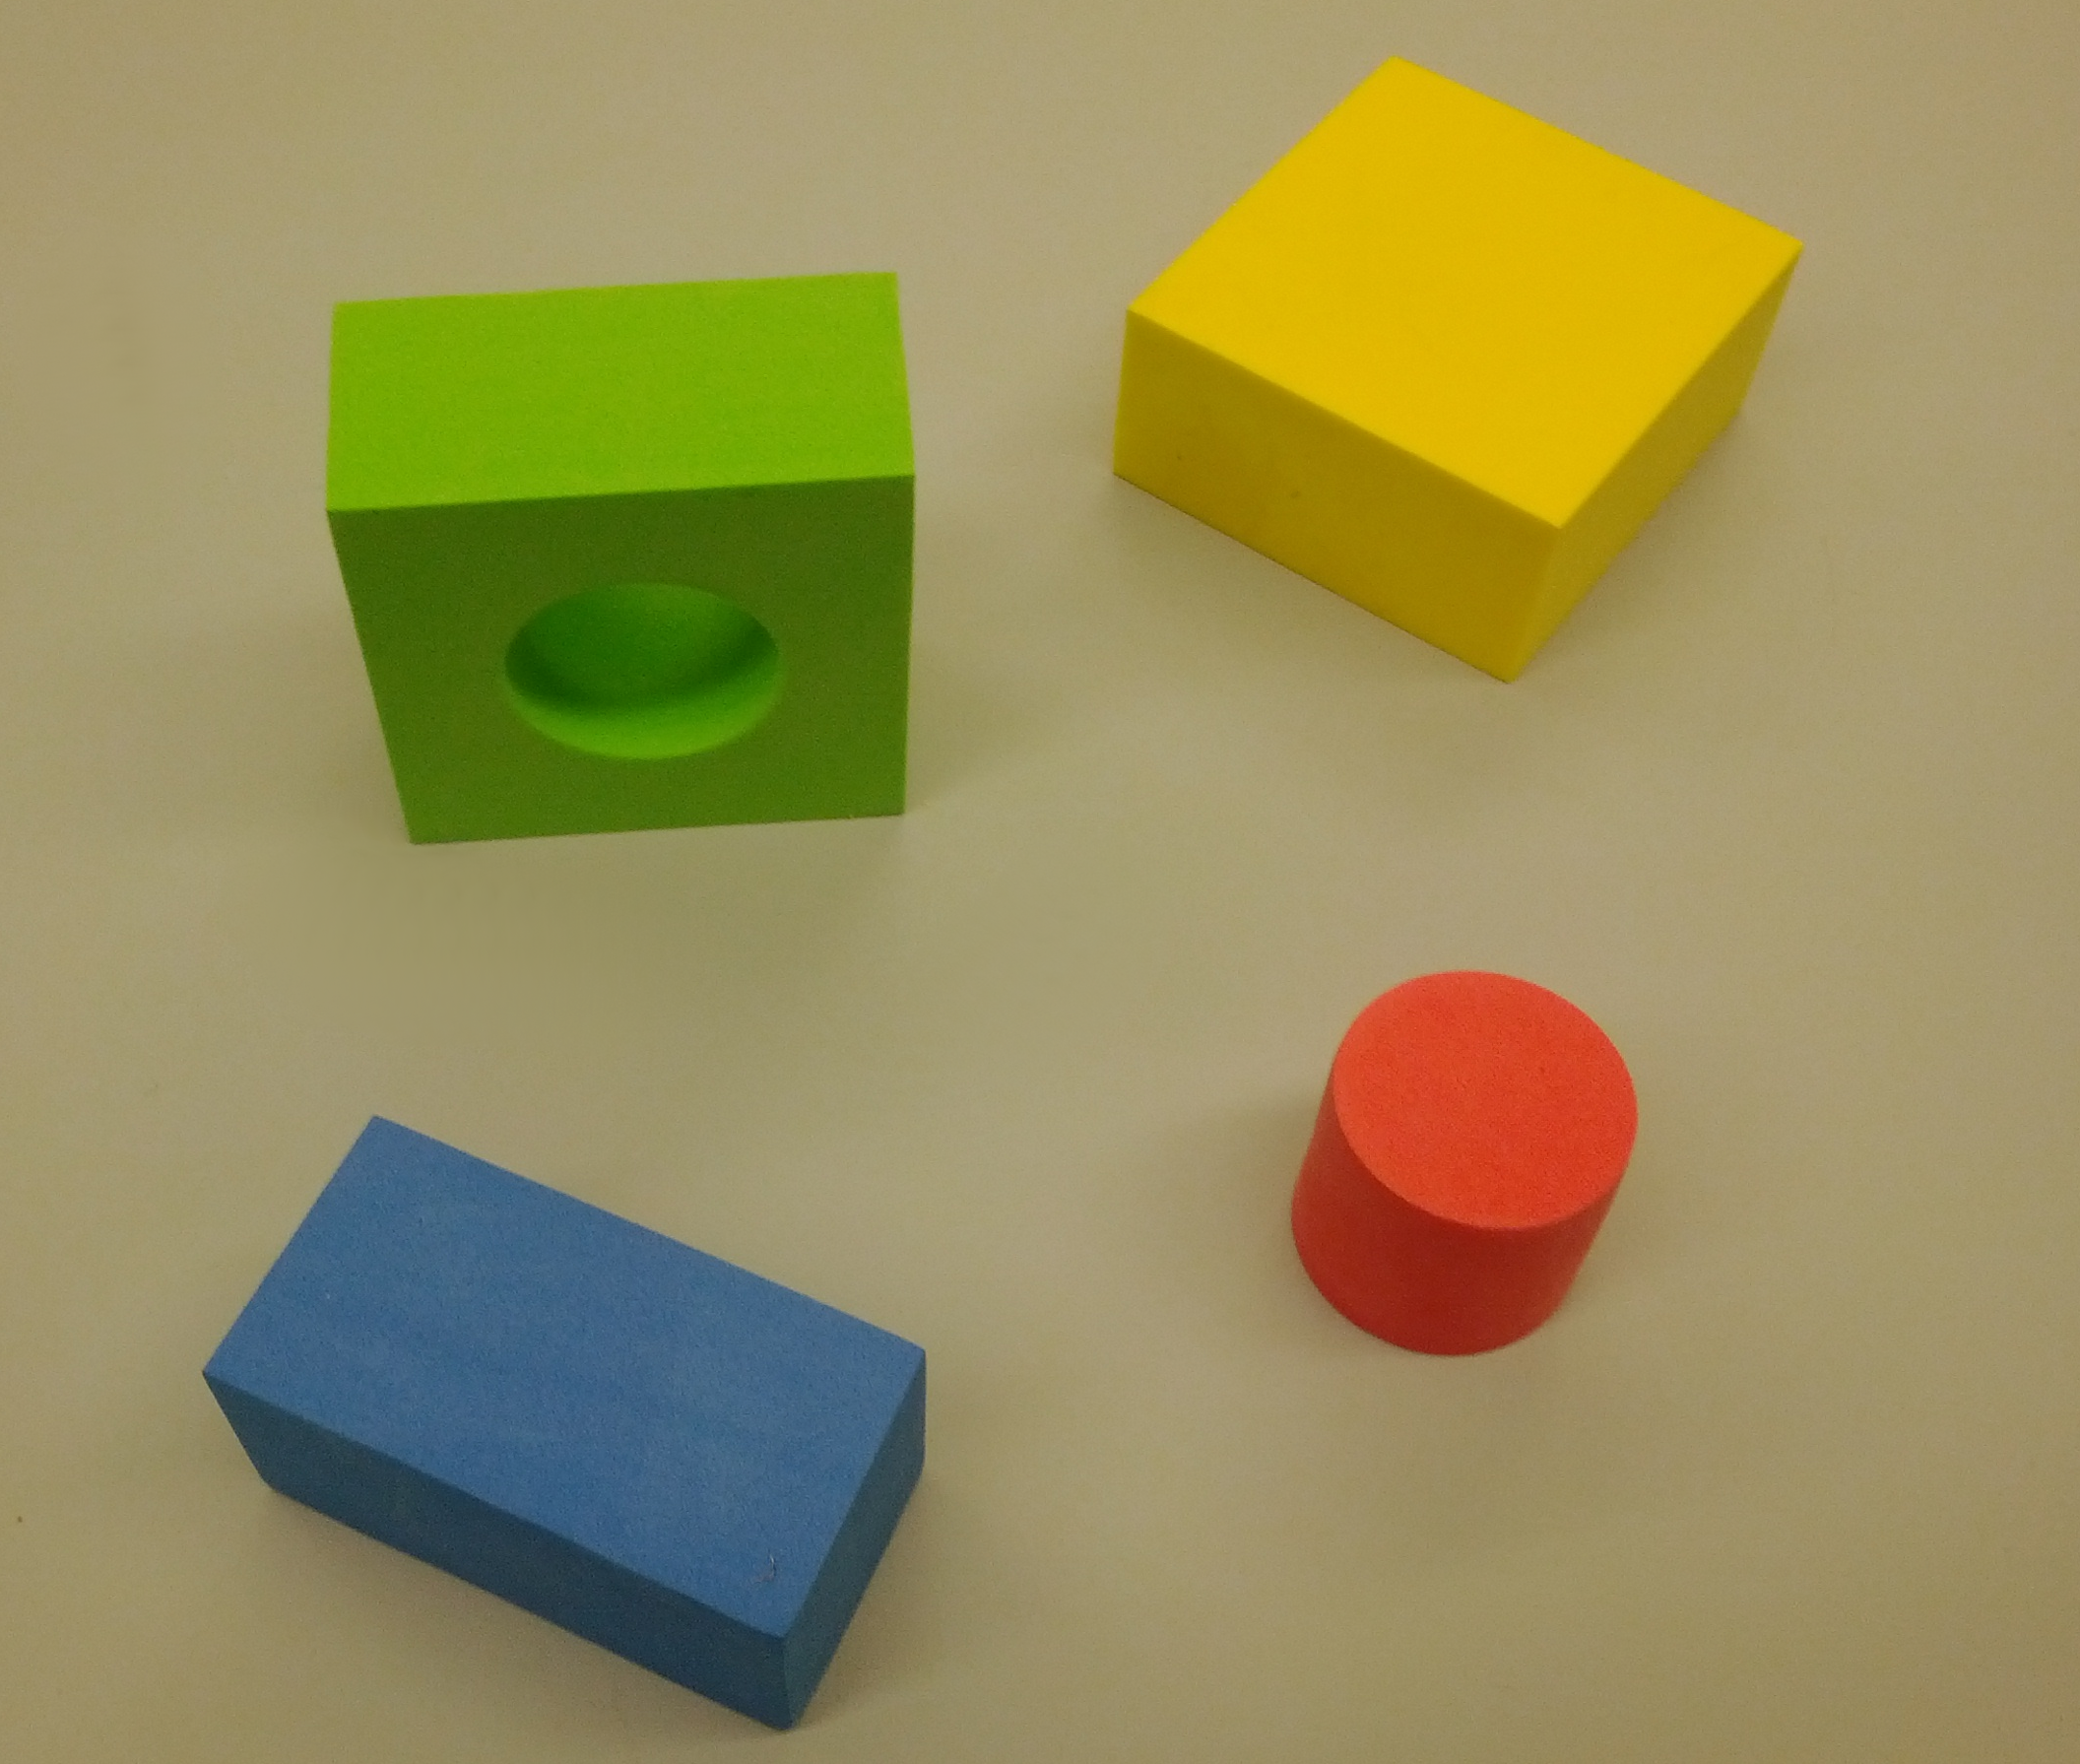
\includegraphics[height=1.6in]{figures/blocks.png}
    \label{fig:blocks}
}
\subfloat[Segmented Images] {
    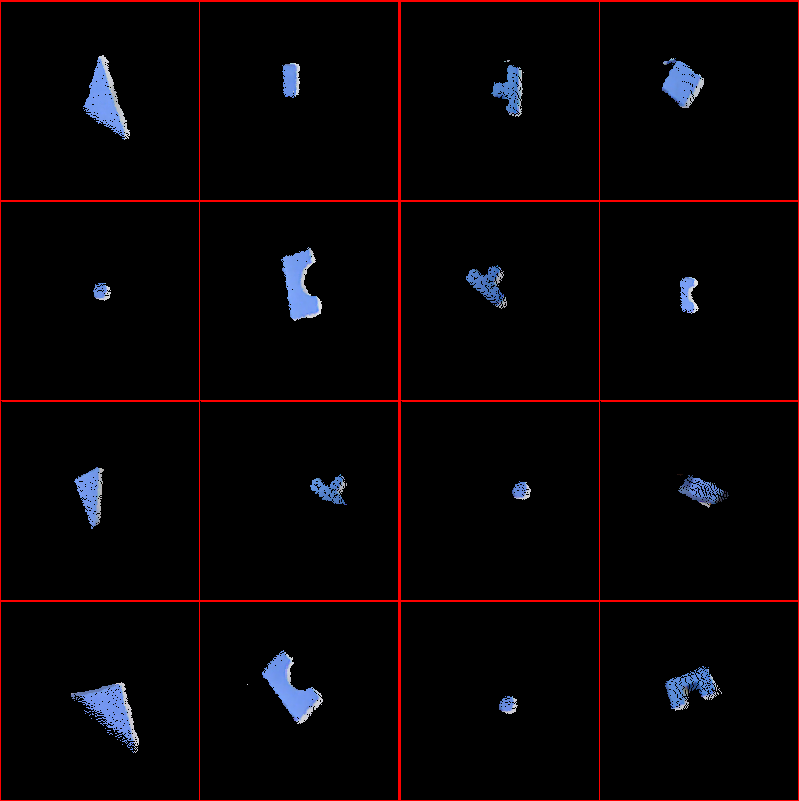
\includegraphics[height=1.6in]{figures/blue_objs.png}
    \label{fig:images}
}
\subfloat[Real-world test data] {
    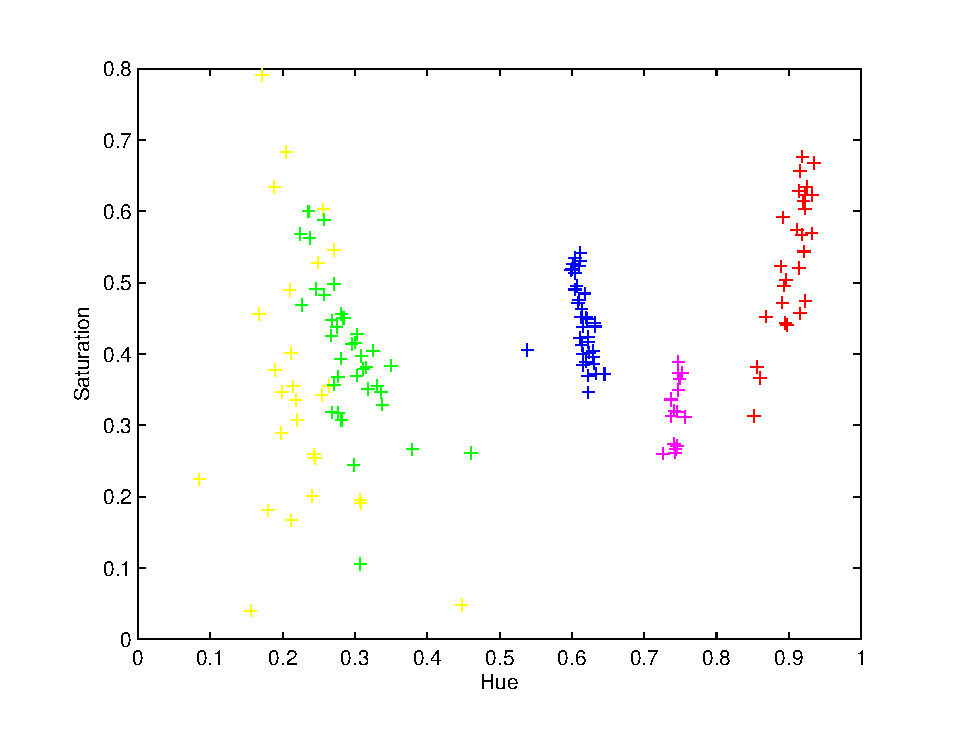
\includegraphics[height=1.6in]{figures/colorplot_noorange.eps}
    \label{fig:colordata}
}
\caption{Real world data is extracted from toy foam blocks. The blocks
    themselves can be seen in \subref{fig:blocks}. Using a segmentation
    algorithm, we extract the blocks from the Kinect data \subref{fig:images}
    and generate feature vectors for each object.
    Finally, we hand label the data for features such as color and shape for
    classification training. In \subref{fig:colordata}, we see the actual
    distribution of our training samples in the hue and saturation
    dimensions.}
\label{fig:objects}
\end{figure}



Initially we used SVM classification to validate our method, but we have since 
moved to a K-nearest neighbor approach.  With the K-nearest neighbor algorithm 
it is easy to add another example to the training, without recreating the 
entire training model as was done with SVM classification.  Additionally we no 
longer rely on third party software, namely liblinear ~\cite{LIBLINEAR} to do 
classification.  Using our implementation of a K-nearest neighbor 
classification we also reported a confidence metric for each label based on the 
percentage of neighbors with a given label.

Testing our system requires direct interaction and presentation of new objects 
or objects at new angles.  Additional testing can be done by training the 
system with new shapes and colors and observing how quickly and effectively it 
can learn and apply the new information.  Qualitatively it is easy to see 
whether the system is performing well.  However to do a less subjective, 
quantitative evaluation of our methodology, we used the leave-one-out-cross-validation 
(LOOCV) method on our collected training data.  This testing method mirrors the 
scenario where a novel object is presented to this system.

The results in Table~\ref{tbl:testresults} \xxx{todo} show LOOCV percentages 
for the shape, color and size.  Unsurprisingly it has more difficulty with shape
, which varies greatly by angle and position, and size, which is a more 
subjective attribute. It has particular problems with shapes that are presented 
head on, which tend to resemble rectangles.  This is the primary motivation for 
developing a confidence threshold learning mechanism, which allows the system 
to determine which labels are inherently uninformative.


% orange 87.10
\begin{table}
\centering
\begin{tabular}{ | l | l | l | l | l | l |}
    \hline
    red &  yellow & green & blue & purple \T \B \\ \hline
    96.43\%  & 92.00\% & 97.37 \% & 100.00\% & 88.57\% \B \T \\ \hline
\end{tabular}
\caption{This shows the result of OVA classification for five color types
    across 160 objects. Each test involved training on 80\% of the points,
           with 20\% left out for testing.}
\label{tbl:testresults}
\end{table}


\section{Conclusion}
%\xxx{Summary of your progress and your final expected goal (what do you expect
%    to achieve or demonstrate for the final project?)}


\bibliographystyle{plain}
\bibliography{literature}

\end{document}

% LocalWords:  multiclass
